\section{Results}\label{sec:results}

\subsection{Logical error per round}\label{sec:eps}

Figure~\ref{fig:eps} shows the logical error per round of the homogeneous (median) circuits. At the calibrated rates
($s = 1$) the error per round falls from $d = 3$ to $d = 5$ on \BelowPmOne{} of the \NumDevices{} devices with PM and
on \BelowCorrOne{} with PM-corr; at $s = 0.5$ and $s = 0.25$ it falls on all of them with every decoder. The two
Heron r3 devices are the lowest at every scale, the three Eagle r3 devices the highest. These are properties of the
calibrations under our noise model, not hardware results, but they set the regime: the snapshots place most devices
near or above threshold for this circuit, and the scaled points place them below it.

\begin{figure}[t]
\centering
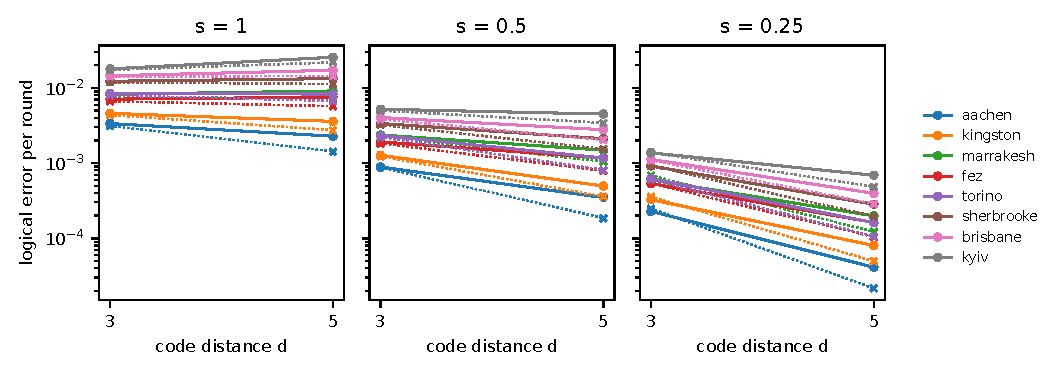
\includegraphics[width=\textwidth]{figures/fig_eps_round.pdf}
\caption{Logical error per round of the median circuits, X and Z pooled. Solid lines: PM; dotted lines: PM-corr.
Panels: error scale $s$.}\label{fig:eps}
\end{figure}

\subsection{The pre-decoder against plain and correlated matching}\label{sec:baselines}

Table~\ref{tab:wins} counts the significant wins and losses of every comparison over all points, and
Fig.~\ref{fig:baselines} shows every failure ratio against the logical error of PM.

\begin{table}[t]
\caption{Paired comparisons over all placements and scales: points where the first decoder fails significantly less
(Better) or more (Worse) often than the second (exact sign test, $p < 0.05$), and the range of failure ratios. The
median weight comparison uses only the best and screened placements, where the two graphs differ.}\label{tab:wins}
\centering
% generated by analysis/summarize.py; do not edit
\begin{tabular}{llrrrr}
\toprule
Comparison & $d$ & Points & Better & Worse & Failure ratio \\
\midrule
INT8 pre-decoder + PM vs PM & 3 & 54 & 35 & 4 & 0.85 to 1.17 \\
INT8 pre-decoder + PM vs PM & 5 & 54 & 44 & 4 & 0.64 to 1.06 \\
INT8 pre-decoder + PM vs PM-corr & 3 & 54 & 21 & 12 & 0.73 to 1.20 \\
INT8 pre-decoder + PM vs PM-corr & 5 & 54 & 0 & 51 & 1.07 to 1.61 \\
float pre-decoder + PM vs PM-corr & 3 & 54 & 17 & 19 & 0.76 to 1.24 \\
float pre-decoder + PM vs PM-corr & 5 & 54 & 0 & 49 & 0.99 to 1.60 \\
float pre-decoder + PM-corr vs PM-corr & 3 & 54 & 20 & 15 & 0.76 to 1.24 \\
float pre-decoder + PM-corr vs PM-corr & 5 & 54 & 0 & 49 & 0.99 to 1.61 \\
PM-corr vs PM & 3 & 54 & 25 & 8 & 0.90 to 1.29 \\
PM-corr vs PM & 5 & 54 & 54 & 0 & 0.50 to 0.87 \\
PM, median weights vs calibrated & 3 & 30 & 0 & 19 & 0.99 to 1.16 \\
PM, median weights vs calibrated & 5 & 30 & 0 & 20 & 0.97 to 1.15 \\
\bottomrule
\end{tabular}

\end{table}

\begin{figure}[t]
\centering
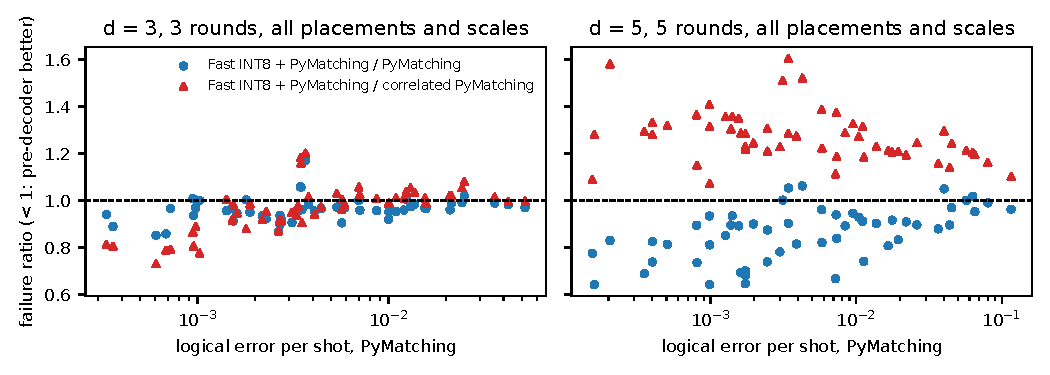
\includegraphics[width=\textwidth]{figures/fig_baselines.pdf}
\caption{Failures of the INT8 pre-decoder followed by PM, divided by the failures of PM (circles) and of PM-corr
(triangles), at every point; X and Z pooled, 400,000 shots per point.}\label{fig:baselines}
\end{figure}

\textbf{Against plain matching} the pre-decoder helps, as NVIDIA reports for uniform noise
\cite{chamberland2026predecoder}: it is significantly better at \PmThreeBetter{} of \PmThreeN{} points at $d = 3$ and
\PmFiveBetter{} of \PmFiveN{} at $d = 5$, with failure ratios down to \PmThreeMin{} and \PmFiveMin{}. The gain is
largest on Aachen, the lowest error device, and smallest on Torino and the Eagle devices, where the ratio approaches
or exceeds 1 at the calibrated rates.

\textbf{Against correlated matching} the result reverses at $d = 5$. PM-corr alone fails less often than the
pre-decoder pipeline at every one of the \CorrFiveN{} points, significantly at \CorrFiveWorse{}, with ratios from
\CorrFiveMin{} to \CorrFiveMax{}. On Aachen at the calibrated rates, for example, PM fails \ExAachenPm{} times in
400,000 shots, the pre-decoder pipeline \ExAachenFast{} and PM-corr \ExAachenCorr{}. PM-corr itself beats PM at every
$d = 5$ point (ratios \CorrPmFiveMin{} to \CorrPmFiveMax{}), and it already corrects most of what the network adds:
of the shots that the pre-decoder pipeline gets right and PM gets wrong, PM-corr gets \OverlapFive{}\% right at
$d = 5$ and \OverlapThree{}\% at $d = 3$. Correlated matching targets faults that flip detectors of both types, such
as Y errors and two qubit gate faults \cite{fowler2013correlated}, which suggests these are a large part of what the
network learned to remove. The float network gives the same picture (Table~\ref{tab:wins}), so this is not an effect of quantization.
Placing the network in front of PM-corr does not help either (\FcCorrFiveBetter{} better,
\FcCorrFiveWorse{} worse at $d = 5$; on Aachen \ExAachenFastCorr{} failures).

At $d = 3$ the picture is mixed. PM-corr is worse than PM at \LowCorrWorse{} of the \LowN{} points at $s = 0.25$, and
there the pre-decoder beats PM-corr significantly at \LowFastBetterCorr{} of them; overall at $d = 3$ the
pre-decoder is better than PM-corr at \CorrThreeBetter{} points and worse at \CorrThreeWorse{}. In this regime,
small codes at low error, the network gains more over plain matching than correlated matching does.

\subsection{Uneven qubits}\label{sec:uneven}

The best placements, whose qubits are all good but differ, behave like the median ones (mean $d = 5$ ratio against
PM \BestFiveMeanRatio{}, against \MedianFiveMeanRatio{} for median). The screened placements draw from most of a
device's spread. On Aachen they still behave like the median ones, but on Kingston the pre-decoder makes plain
matching significantly worse at \KingScreenWorse{} of \KingScreenN{} points, with ratios up to \KingScreenMax{};
these are most of the significant losses in Table~\ref{tab:wins}, the others being Torino and Sherbrooke at the
calibrated rates. A network trained on uniform noise removes errors as if every location were equally likely. When
the rates of the locations differ widely, some of those removals are wrong, while PM, which weights each edge by its
own rate, is not misled in the same way. We read this as a limit of the training distribution rather than of
pre-decoding, which training on calibrated noise could test.

\subsection{Calibrated matching weights}\label{sec:weights}

On the best and screened placements the calibrated circuit and the median circuit differ, and PM can be given
either graph. Figure~\ref{fig:weights} shows the failure ratio of the median graph to the calibrated one. Median
weights are never significantly better, and are significantly worse at \MedWThreeWorse{} of \MedWThreeN{} points at
$d = 3$ and \MedWFiveWorse{} of \MedWFiveN{} at $d = 5$ (Table~\ref{tab:wins}), by up to \MedWeightsMax{} times. This gain needs
no network and no accelerator, only the calibration file, and it is of the same size as the network's gain over PM
at $d = 3$.

\begin{figure}[t]
\centering
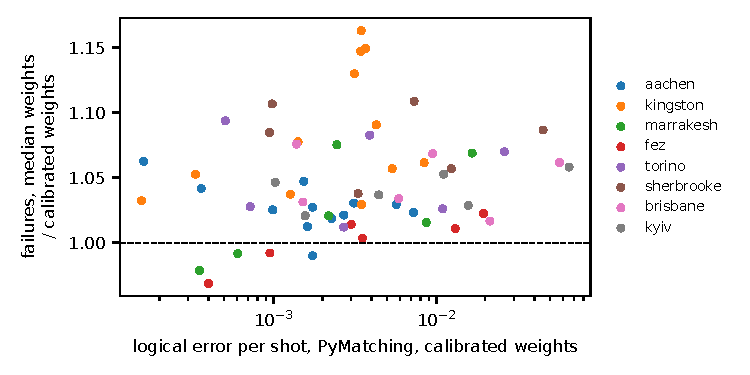
\includegraphics[width=0.75\textwidth]{figures/fig_weights.pdf}
\caption{Failures of PM with the device median graph divided by failures of PM with the calibrated graph, best and
screened placements, against the logical error of the calibrated PM.}\label{fig:weights}
\end{figure}

\subsection{One U55C card}\label{sec:cardres}

Table~\ref{tab:card} lists the \CardConfigs{} card runs. Both kernel instances were bit exact against the integer
model in \CardAllExact{} runs, and in all \CardCompared{} runs that have a CPU integer counterpart the set of shots
on which the card pipeline fails is identical to that of the CPU integer model. The $d = 7$ runs on
Kingston, outside the CPU campaign, show no gain over PM at that distance: the card pipeline fails more often than
PM in three of the four runs.

\begin{table}[t]
\caption{Card runs: logical failures of PM and of the card's INT8 decisions followed by PM on the same 200,000 shots,
and whether the failing shots equal those of the CPU integer model (n/a: no CPU integer run at that
point).}\label{tab:card}
\centering
% generated by analysis/summarize.py; do not edit
\begin{tabular}{lrrlrrrl}
\toprule
Device & Scale & $d$ & Basis & Shots & PM & Card + PM & Same as CPU \\
\midrule
Kingston & 1 & 3 & X & 200,000 & 3,789 & 3,659 & yes \\
Kingston & 1 & 3 & Z & 200,000 & 1,677 & 1,721 & yes \\
Kingston & 1 & 5 & X & 200,000 & 5,257 & 4,847 & yes \\
Kingston & 1 & 5 & Z & 200,000 & 1,820 & 1,637 & yes \\
Kingston & 1 & 7 & X & 200,000 & 5,286 & 5,517 & n/a \\
Kingston & 1 & 7 & Z & 200,000 & 1,355 & 1,409 & n/a \\
Kingston & 0.5 & 3 & X & 200,000 & 1,050 & 1,026 & yes \\
Kingston & 0.5 & 3 & Z & 200,000 & 472 & 472 & yes \\
Kingston & 0.5 & 5 & X & 200,000 & 741 & 658 & yes \\
Kingston & 0.5 & 5 & Z & 200,000 & 246 & 205 & yes \\
Kingston & 0.5 & 7 & X & 200,000 & 432 & 483 & n/a \\
Kingston & 0.5 & 7 & Z & 200,000 & 97 & 88 & n/a \\
Aachen & 1 & 3 & X & 200,000 & 1,898 & 1,757 & yes \\
Aachen & 1 & 3 & Z & 200,000 & 2,105 & 1,925 & yes \\
Aachen & 1 & 5 & X & 200,000 & 2,133 & 1,562 & yes \\
Aachen & 1 & 5 & Z & 200,000 & 2,387 & 1,785 & yes \\
Sherbrooke & 0.5 & 3 & X & 200,000 & 2,284 & 2,164 & yes \\
Sherbrooke & 0.5 & 5 & X & 200,000 & 2,407 & 2,245 & yes \\
\bottomrule
\end{tabular}

\end{table}

Table~\ref{tab:perf} gives throughput and latency. One card decodes \CardRateDd{} windows per second at $d = 3$ and
\CardRateDf{} at $d = 5$; a single window takes \CardLatDd{} and \CardLatDf{} ms through PCIe. The float network on
\CpuThreads{} CPU threads is faster at every distance measured, by \CpuOverCardDd{} times at $d = 3$ and
\CpuOverCardDj{} times at $d = 9$, the gap narrowing as the windows grow. At milliseconds per window, neither is
close to the microsecond syndrome cycle of superconducting devices.

\begin{table}[t]
\caption{Throughput of one card (both kernel instances) and latency of one window, against the float network on the
CPU host (forward pass only, batches of 4,096).}\label{tab:perf}
\centering
% generated by analysis/summarize.py; do not edit
\begin{tabular}{rrrrr}
\toprule
$d$ & Card (windows/s) & One window (ms) & CPU (windows/s) & CPU / card \\
\midrule
3 & 4,201 & 1.05 & 21,289 & 5.1 \\
5 & 2,330 & 1.50 & 5,595 & 2.4 \\
7 & 1,171 & 2.34 & 2,082 & 1.8 \\
9 & 622 & 3.84 & 1,016 & 1.6 \\
11 & 360 & 6.21 & n/a & n/a \\
13 & 224 & 9.56 & n/a & n/a \\
\bottomrule
\end{tabular}

\end{table}
